\documentclass[palatino,nosec,nochap,nobuilddate]{Docencia}
\usetikzlibrary[patterns]


\title{Corrección 2º parcial - 2ª evaluación}
\author{Departamento de Matemáticas}
\date{19/20}


% Paquetes adicionales

\usepackage[author={Víctor de Juan, 2020}]{pdfcomment}

\makeatletter
\newcommand{\annotate}[2][]{%
\pdfstringdef\x@title{#1}%
\edef\r{\string\r}%
\pdfstringdef\x@contents{#2}%
\pdfannot
width 2\baselineskip
height 2\baselineskip
depth 0pt
{
/Subtype /Text
/T (\x@title)
/Contents (\x@contents)
}%
}
\makeatother



\usepackage{eso-pic}
\newcommand\BackgroundPic{%
\put(0,0){%
\parbox[b][\paperheight]{\paperwidth}{%
\vfill
\centering
%\includegraphics[width=\paperwidth,height=\paperheight,%
%keepaspectratio]{../../../../BWLogo.jpeg}%
\vfill
}}}





\begin{abstract}
Corrección del 2º examen de la 2ª evaluación de Matemáticas I, curso 2019-2020.

\nota{No está exento de erratas. En caso de descubrir alguna, por favor, comunicarlas al autor.}
\end{abstract}

% --------------------
\newcommand{\cimplies}{\text{\hl{$\implies$}}}
\renewcommand{\vec}[1]{\overrightarrow{#1}}

\usepackage{tikz}
\usepackage{tikz-3dplot}

\usetikzlibrary{calc,patterns,angles,quotes}
\begin{document}
\pagestyle{plain}
\maketitle

\AddToShipoutPicture{\BackgroundPic}

\newpage
\begin{problem}
Desde una posición ves a un buitre que vuela, según tus cálculos, a unos 120m de altura. Ves al buitre con un ángulo respecto de la horizontal de 60º. Si bajas la mirada hasta los 30º, manteniendo la dirección, observas que vuela una perdiz a unos 100m de altura. ¿Qué distancia aproximadamente les separa?
\solution


\begin{figure}[hbtp]
\centering

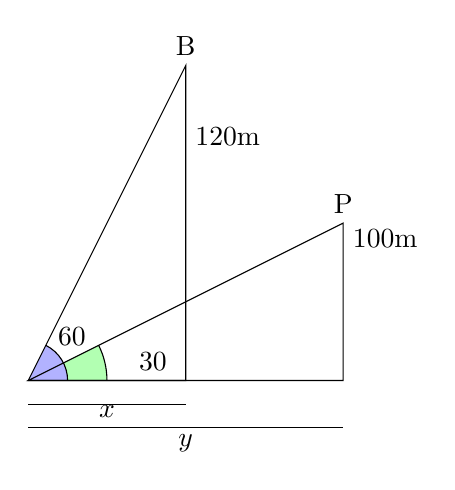
\begin{tikzpicture}[]
    % draw axes
\coordinate (a) at (0,0);
\coordinate (b) at (4,0);
\coordinate (e) at (2,0);
\coordinate (c) at (2,4);
\coordinate (d) at (4,2);

\draw pic[draw,fill=green!30,angle radius=1cm,"$30º$" shift={(10mm,1mm)}] {angle=b--a--d};
\draw pic[draw,fill=blue!30,angle radius=0.5cm,"$60º$" shift={(3mm,4mm)}] {angle=e--a--c};

\draw  (a) -- (b) -- (d) -- cycle;
\draw  (a) -- (e) -- (c) -- cycle;

\draw (c) node[anchor=south]{B};
\draw (d) node[anchor=south]{P};
\draw (4,1.8) node[anchor=west]{100m};
\draw (2,3.1) node[anchor=west]{120m};
\draw (0,-0.3) -- (2,-0.3);
\draw (1,-0.4) node{$x$}; 
\draw (0,-0.6) -- (4,-0.6);
\draw (2,-0.8) node{$y$}; 
\end{tikzpicture}
\end{figure}

\[\tg(60) = \frac{120}{x} \implies x=\frac{120}{\tg(60)} = 69.28m \]

\[\tg(30) = \frac{100}{y} \implies y = \frac{100}{\tg(30)} =  173.21m\]

Consideremos el triángulo azul, donde $y-x = 103.92$


\begin{figure}[hbtp]
\centering

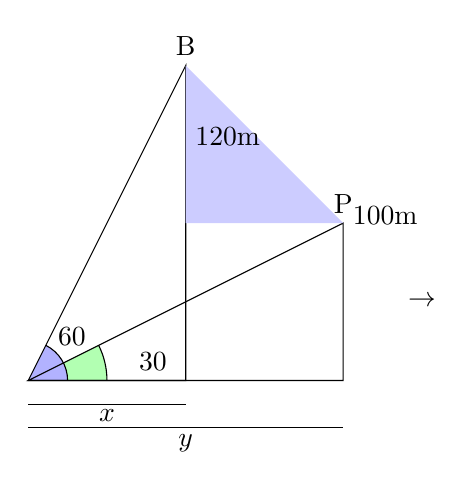
\begin{tikzpicture}    % draw axes
\coordinate (a) at (0,0);
\coordinate (b) at (4,0);
\coordinate (e) at (2,0);
\coordinate (c) at (2,4);
\coordinate (d) at (4,2);
\coordinate (v) at (2,2);

\draw pic[draw,fill=green!30,angle radius=1cm,"$30º$" shift={(10mm,1mm)}] {angle=b--a--d};
\draw pic[draw,fill=blue!30,angle radius=0.5cm,"$60º$" shift={(3mm,4mm)}] {angle=e--a--c};

\draw  (a) -- (b) -- (d) -- cycle;
\draw  (a) -- (e) -- (c) -- cycle;
\fill[blue!20] (d) -- (c) -- (v);

\draw (c) node[anchor=south]{B};
\draw (d) node[anchor=south]{P};
\draw (4,2.1) node[anchor=west]{100m};
\draw (2,3.1) node[anchor=west]{120m};
\draw (0,-0.3) -- (2,-0.3);
\draw (1,-0.45) node{$x$}; 
\draw (0,-0.6) -- (4,-0.6);
\draw (2,-0.8) node{$y$}; 
\draw (5,1) node{$\to$};
\end{tikzpicture} 
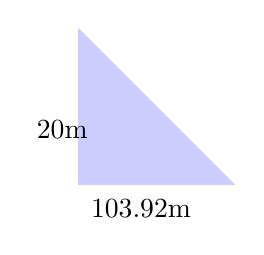
\begin{tikzpicture}    % draw axes
\coordinate (a) at (1,3);
\coordinate (b) at (5,3);
\coordinate (e) at (3,3);
\coordinate (c) at (3,7);
\coordinate (d) at (5,5);
\coordinate (v) at (3,5);

%\draw pic[draw,fill=green!30,angle radius=1cm,"$30º$" shift={(10mm,1mm)}] {angle=b--a--d};
%\draw pic[draw,fill=blue!30,angle radius=0.5cm,"$60º$" shift={(3mm,4mm)}] {angle=e--a--c};

\fill[blue!20] (d) -- (c) -- (v) -- cycle;
\draw (3.8,4.7) node{103.92m};
\draw (2.8,5.7) node{20m};

\end{tikzpicture}
\end{figure}

Se calcula la hipotenusa del triángulo azul con Pitágoras.

\[
d(P,B) = \sqrt{20^2 + 103.92^2} = 105.83\text{m}
\]

\end{problem}

\begin{problem} Resuelve el siguiente sistema:

\[
\left\{\begin{array}{c}
\sen(2x) + \sen(2y) = \frac{\sqrt{3}+1}{2}\\
\sen(2x) - \sen(2y) = \frac{\sqrt{3}-1}{2}
\end{array}\right\} \implies 
\]
\solution
\[
\left\{\begin{array}{ll}
E_1+E_2: &2\sen(2x) = \frac{\sqrt{3}+1}{2} + \frac{\sqrt{3}-1}{2} = \sqrt{3} \dimplies \sen(2x) = \rfrac{\sqrt{3}}{2}\\
E1-E_2: &2\sen(2y) = \frac{\sqrt{3}+1}{2} - \frac{\sqrt{3}-1}{2} = 1 \dimplies \sen(2y) = \rfrac{1}{2}
\end{array}\right\} 
\]

Resolvemos:

\[
	\sen(2x) = \rfrac{\sqrt{3}}{2} \to 2x = \frac{\pi}{3}+2\pi k \dimplies x = \left\{ \frac{\pi}{6}+\pi·k , k\in\mathbb{Z}\right\}
\]

\[
	\sen(2y) = \rfrac{1}{2} \to 2y = \frac{\pi}{6}+2\pi k \dimplies y = \left\{ \frac{\pi}{12}+\pi·k , k\in\mathbb{Z}\right\}
\]

La solución del sistema será:

\[
(x,y) = \left(\frac{\pi}{6}+\pi·k,\frac{\pi}{12}+\pi·k \right), k\in\mathbb{Z} 
\]

\end{problem}

\begin{problem}
Dado el siguiente sistema:
\ppart Discute en función del parámetro $a$.
\ppart Resuelve para $a=2$.

\[
\left\{
	\begin{array}{c}
		-x+y-2z=-1\\
		-3x+ay+4z=4\\
		-x+y+3z=4
	\end{array}
\right\}
\]

\solution
\spart 
\[
\left\{
	\begin{array}{c}
		-x+y-2z=-1\\
		-3x+ay+4z=4\\
		-x+y+3z=4
	\end{array}
\right\}\dimplies
\left\{
	\begin{array}{c}
		-x-2z+y=-1\\
		-x+3z+y=4\\
		-3x+4z+ay=4
	\end{array}
\right\}\overset{E_2' = E_1-E_2}{\dimplies}
\left\{
	\begin{array}{c}
		-x-2z+y=-1\\
		-5z=-5\\
		-3x+4z+ay=4
	\end{array}
\right\}\overset{E_3' = 3E_1-E_2}{\dimplies}
\]
\[
\left\{
	\begin{array}{c}
		-x-2z+y=-1\\
		-5z=-5\\
		10z+(a-3)y=7
	\end{array}
\right\}{E_3' = 2E_2+E_3}{\dimplies}
\left\{
	\begin{array}{r}
		-x-2z+y=-1\\
		-5z+0y=-5\\
		(a-3)y=-3
	\end{array}
\right\}
\]

\textbf{Discusión:}
\begin{itemize}
	\item Si $a=3$ el sistema es incompatible por contener la ecuación $0y=-3$.
	\item Si $a\neq 3$, el sistema es compatible indeterminado porque es un sistema escalonado con el mismo número de ecuaciones que de incógnitas.
\end{itemize}

\spart 
\[
\left\{
	\begin{array}{r}
		-x-2z+y=-1\\
		-5z+0y=-5\\
		-y=-3
	\end{array} \dimplies
\right\}\dimplies
\left\{
	\begin{array}{r}
		-x-2z+y=-1\\
		z=1\\
		y=3
	\end{array} -x-2+3=-1 \dimplies x=0
\right\}
\]

\end{problem}


\begin{problem}

Sea $z=1-i$.
\ppart $z^6$
\ppart $\sqrt[5]{z}$

\solution

Pasamos a polares: 
\begin{itemize}
	\item $\arg(z) \to \arctg\frac{1}{1} = \rfrac{\pi}{4}$. Dado que $z\in II$, $\arg(z) = -\rfrac{\pi}{4}$
	\item $|z| = \sqrt{2}$
\end{itemize}

\[z = 1-i = \sqrt{2}_{\rfrac{-\pi}{4}}\]

\spart

\[|z^6| = \left(\sqrt{2}\right)^6 = 8\]
\[\arg(z^6) = \rfrac{-\pi}{4}·6 = \frac{\pi}{2}\]

Por lo tanto, $z^6 = 8_{\rfrac{\pi}{2}} = 8i$

\spart 
\[\sqrt[5]{z} = \left\{ \sqrt[5]{\sqrt{2}}_{\displaystyle\frac{-\rfrac{\pi}{4}+2\pi k}{5}} \right\}\]
\begin{itemize}
	\item $k=1$
	\[z_1 = \sqrt[10]{2}_{\displaystyle\frac{-\rfrac{\pi}{4}+2\pi ·1}{5}} = \sqrt[10]{2}_{\displaystyle\rfrac{3\pi}{20}}\]
	\item $k=2$
	\[z_2 = \sqrt[10]{2}_{\displaystyle\frac{-\rfrac{\pi}{4}+2\pi ·2}{5}} = \sqrt[10]{2}_{\displaystyle\rfrac{7\pi}{20}}\]
	\item $k=3$
	\[z_3 = \sqrt[10]{2}_{\displaystyle\frac{-\rfrac{\pi}{4}+2\pi ·3}{5}} = \sqrt[10]{2}_{\displaystyle\rfrac{11\pi}{20}}\]
	\item $k=4$
	\[z_4 = \sqrt[10]{2}_{\displaystyle\frac{-\rfrac{\pi}{4}+2\pi ·4}{5}} = \sqrt[10]{2}_{\displaystyle\rfrac{15\pi}{20}}\]
	\item $k=5$
	\[z_5 = \sqrt[10]{2}_{\displaystyle\frac{-\rfrac{\pi}{4}+2\pi ·5}{5}} = \sqrt[10]{2}_{\displaystyle\rfrac{19\pi}{20}}\]
\end{itemize}


\end{problem}

\end{document}